\chapter{Examples}
Ein paar Beispiele, die ich spaeter in die Kapitel reinstelle. 

\begin{exam}
	\label{Ex:ex2}
	\begin{align}
	A = \begin{pmatrix}
	-.5 & 0 \\ 0 & -.3
	\end{pmatrix},
	\begin{pmatrix}   
	0 \\ 0
	\end{pmatrix}, N = 200. 
	\end{align}
	\begin{figure}[ht]
		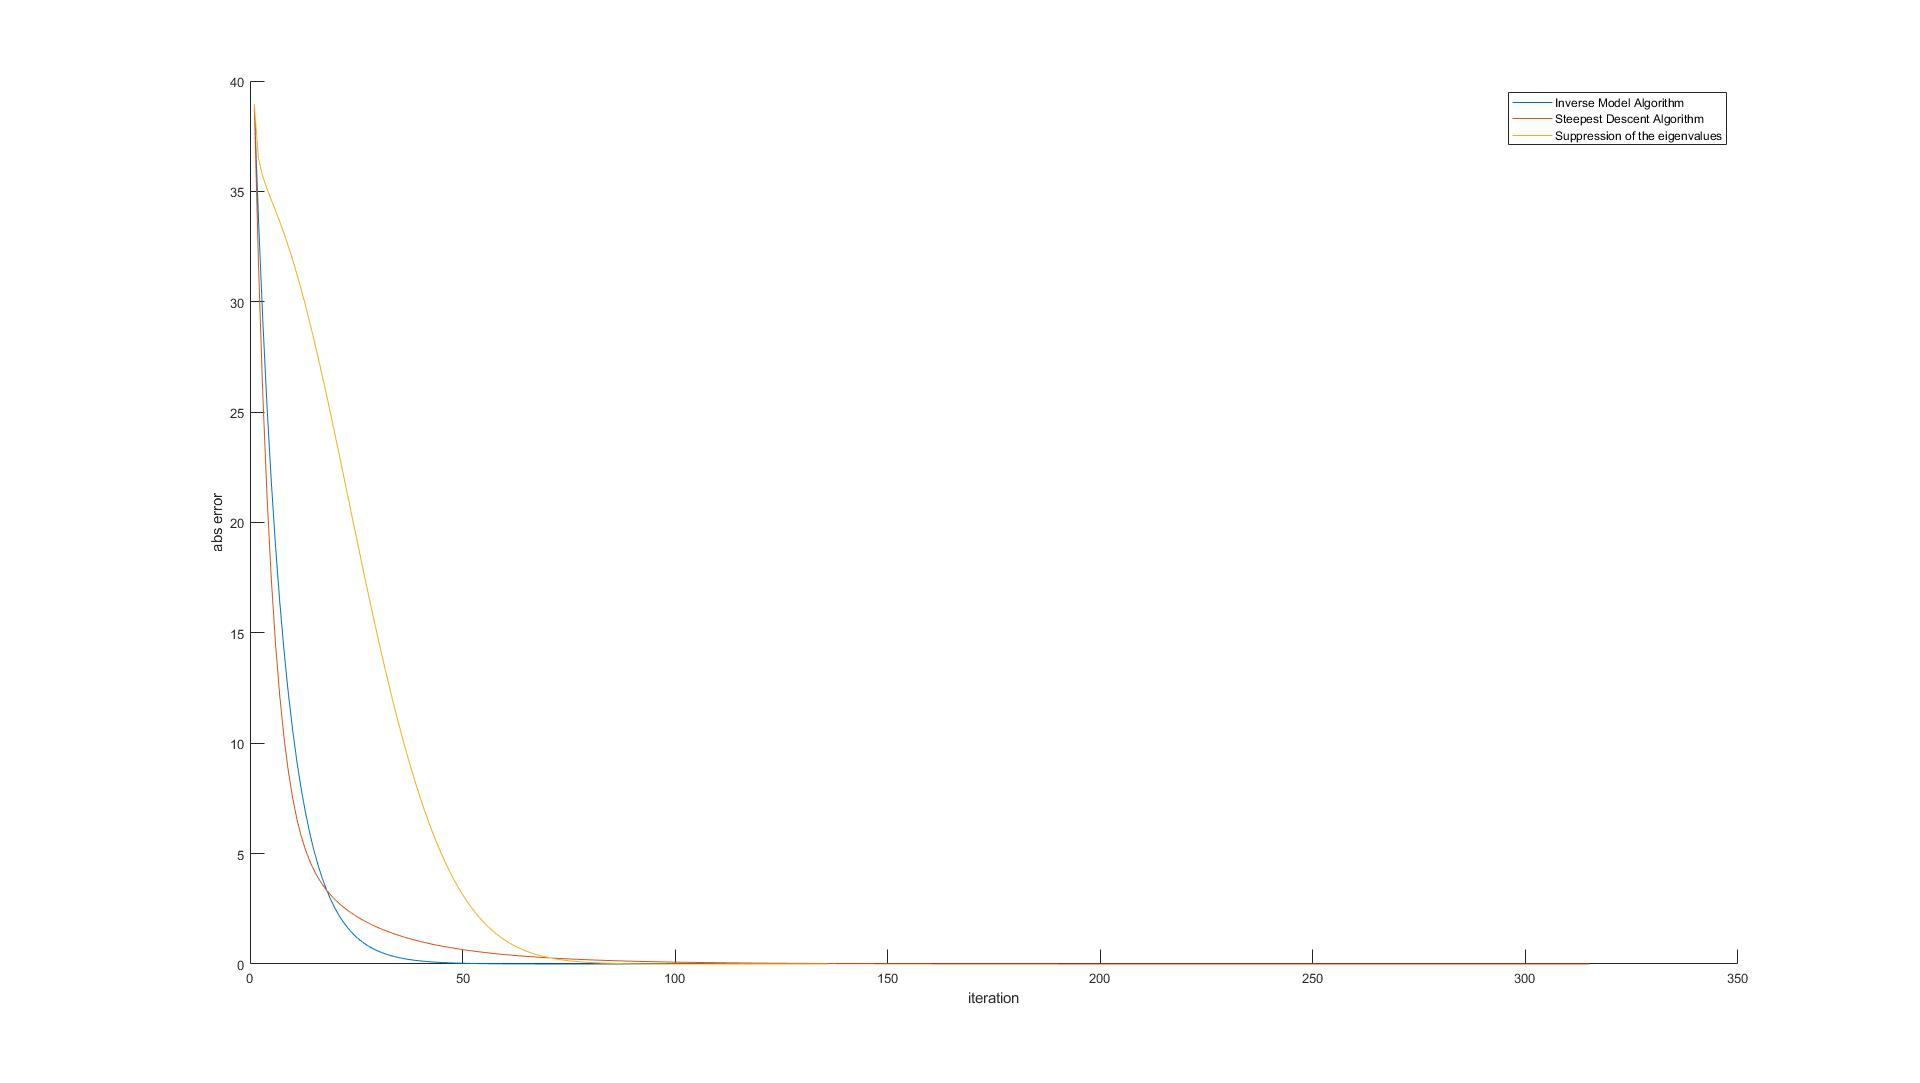
\includegraphics[width=\textwidth]{fig/Ex2.jpg}
		\caption{Example \ref{Ex:ex2}. $u_0 = .1$, $r(t)$ is random for $t = 0, 1, 2, \dots, N$.}
	\end{figure}	
\end{exam}

\begin{exam}
	Satellite Example
	\begin{figure}[ht]
		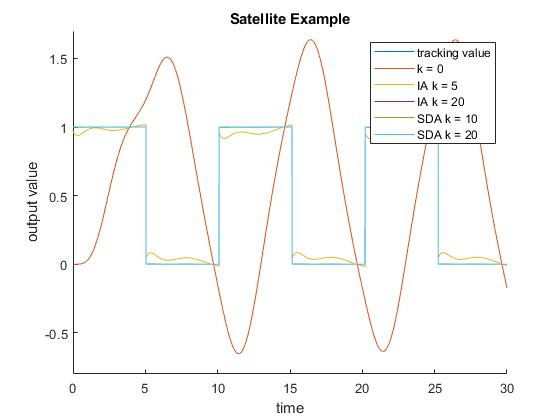
\includegraphics[width=\textwidth]{fig/SatelliteEx.jpg}
		\caption{}
	\end{figure}	
\end{exam}

\begin{exam}
	\label{ex:Unc}
	Uncertain Example
	\begin{align}
	A = \begin{pmatrix}
	-.5 + a & 0 \\ 0 & -.4-a
	\end{pmatrix}, 
	B = \begin{pmatrix}
	1 \\ 1
	\end{pmatrix}, 
	C = \begin{pmatrix}
	.1 & .2
	\end{pmatrix},
	D = 1. x_0 = \begin{pmatrix}
	0 \\ 0
	\end{pmatrix}, N = 200. 
	\end{align}
	$a$ is an uncertain parameter with nominal value $\hat{a} = 1.5$ and variability $a \in [1.3, \; 1.8]$.
	\begin{figure}[ht]
		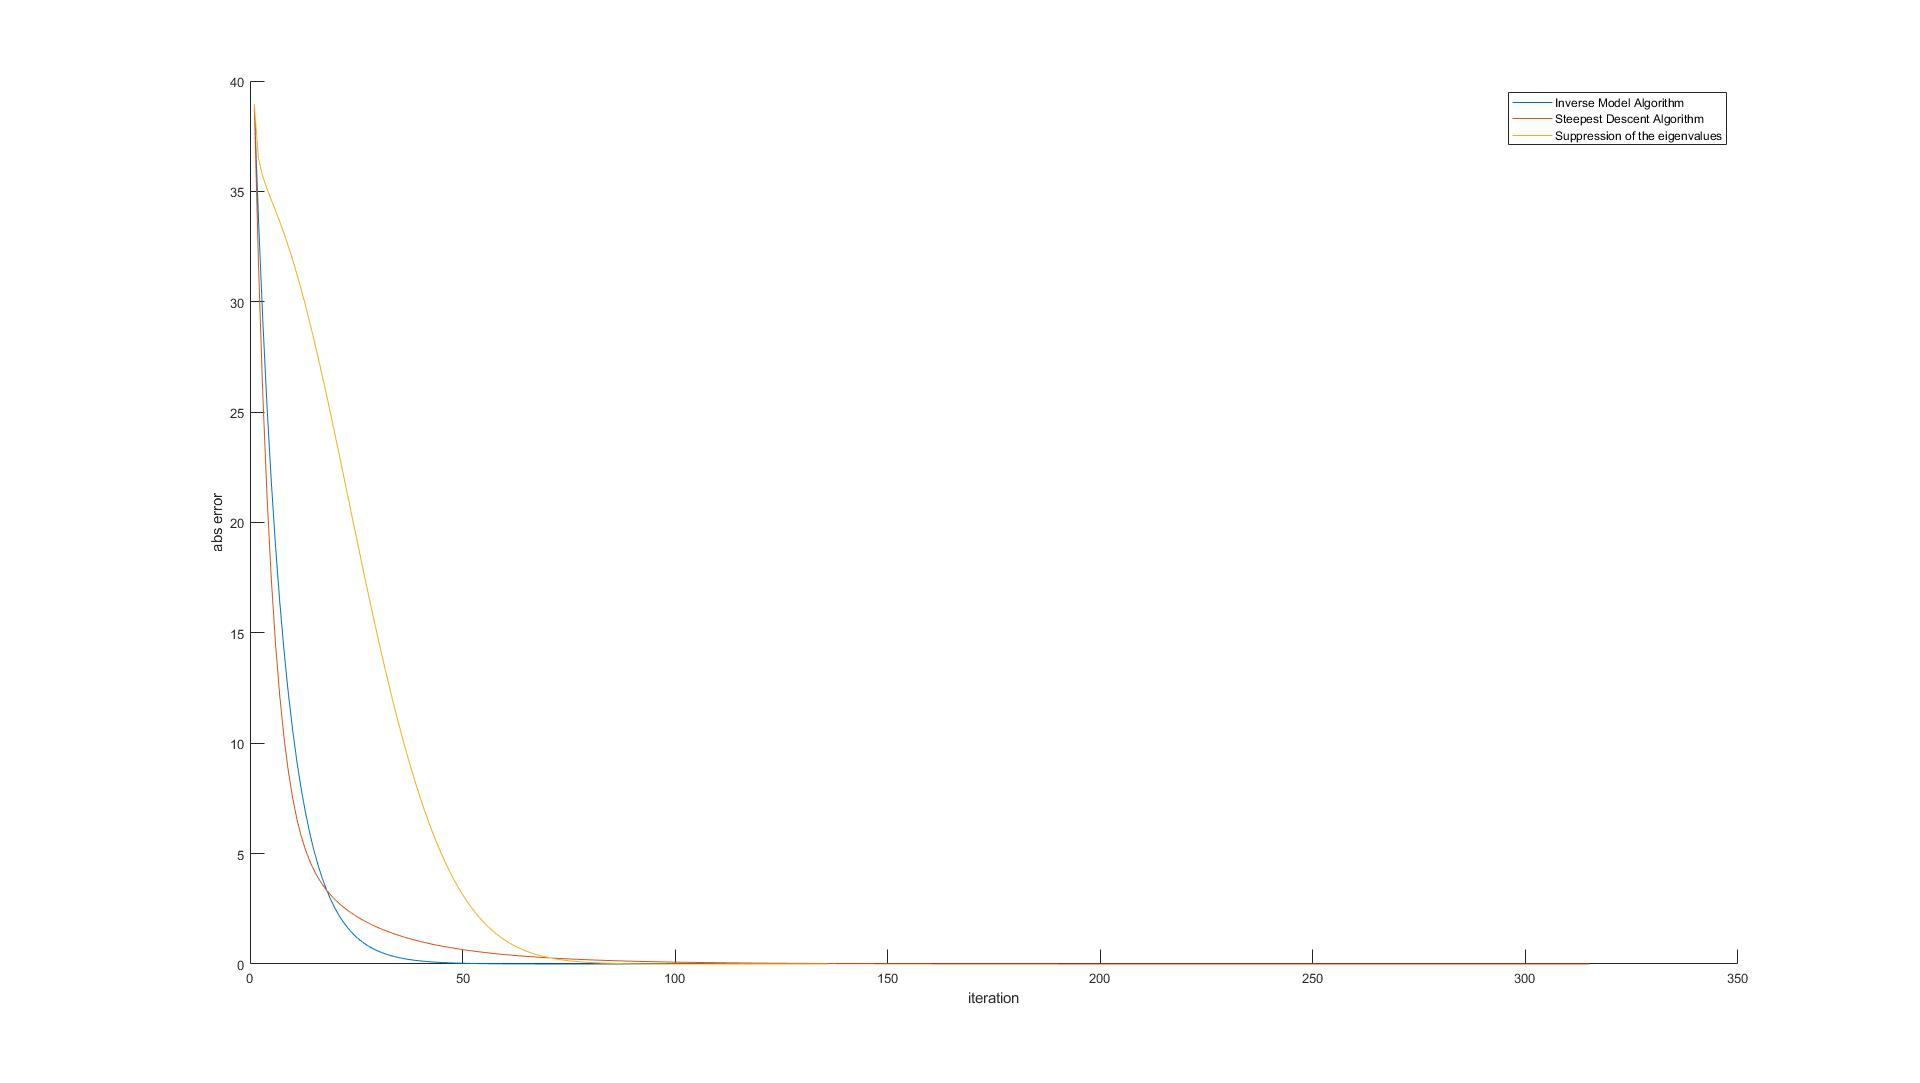
\includegraphics[width=\textwidth]{fig/Ex2.jpg}
		\caption{Example \ref{ex:Unc}. $u(0) = .1$, $r(t)$ is random for $t = 0, 1, 2, \dots, N$.}
	\end{figure}	
\end{exam}